\chapter{Risultati}
In questo capitolo si presentano i risultati della fase sperimentale effettuata su tutti i sistemi mostrati precedentemente: classificatore \textit{random forest}, classificatore neurale, autoencoder e GAN. Le metriche di valutazione utilizzate sono enunciate all'interno della sezione \ref{metriche}. In sezione \ref{res:crf} vengono mostrati i risultati sperimentali ottenuti dal classificatore random forest, punto di partenza di questo studio. In sezione \ref{ris:cnn} vengono mostrati i risulati sperimentali ottenuti dal classificatore neurale, evoluzione del classificatore random forest, e le problematiche incontrate durante tale fase. In sezione \ref{ris:autoenc} viene mostrata la fase sperimentale che ha coinvolto l'autoencoder, per durante la quale si sono ottenuti i pesi utilizzati successivamente come punto di partenza per la fase di training della Generative Adversarial Network. All'interno dell'ultima sezione ( \ref{ris:gan} ) sono mostrati i risultati ottenuti dal training della GAN e la lunga fase di tuning richiesta da quest'ultima.

\pagebreak
\section{Metriche di valutazione}
\label{metriche}
Le metriche di valutazione utilizzate per testare la qualità dei modelli sono state:
\begin{itemize}
\item \textbf{Precision}: il rapporto $\frac{t_p}{t_p+f_p}$ dove $t_p$ è il numero di veri positivi e $f_p$ il numero di falsi positivi. Intuitivamente è l'abilità del classificatore di non marcare come positivo un campione negativo.
\item \textbf{Recall}: il rapporto $\frac{t_p}{t_p+f_n}$  dove $f_n$ sono i falsi negativi. Intuitivamente è l'abilità del classificatore di trovare tutti i campioni positivi.
\item \textbf{F-score}: è definito come la media armonica tra \textit{precision} e \textit{recall}: 
\[F_1 = 2 \cdot \frac{1}{\tfrac{1}{\mathrm{recall}} + \tfrac{1}{\mathrm{precision}}} = 2 \cdot \frac{\mathrm{precision} \cdot \mathrm{recall}}{\mathrm{precision} + \mathrm{recall}}\]
\item \textbf{Area sottesa da Receiver Operating Characteristic}:  metodo grafico per la valutazione della qualità di un classificatore binario al variare della soglia di discriminazione. E' creata graficando la frazione dei veri positivi rispetto ai campioni positivi ($tpr$ = True positive rate) contro la frazione dei falsi positivi rispetto ai campioni negativi ($fpr$ = False positive rate). L'area sottesa dalla curva ROC equivale alla probabilità che il classificatore predica un campione positivo casuale rispetto ad un campione negativo casuale. Formalmente è definita da:
\[ A = \int_{\infty}^{-\infty} \mbox{TPR}(T) \left(-\mbox{FPR}'(T)\right) \, dT = \int_{-\infty}^{\infty} \int_{-\infty}^{\infty} I(T'>T)f_1(T') f_0(T) \, dT' \, dT = P(X_1 > X_0)\]
dove 
$X_{1}$ è il punteggio per un'istanza positiva e $X_{0}$ è il punteggio per un'istanza negativa, mentre $f_{0}$ e $f_{1}$ sono densità di probabilità che un campione sia negativo ($1$) o positivo ($0$)
\end{itemize}

\newpage
\section{Classificatore Random Forest}
\label{res:crf}
Il classificatore Random Forest è stato testato in diverse configurazioni. La configurazione che è stata presentata nella sezione \ref{imp:randomforest} ha mostrato i migliori risultati in ogni test.

Il classificatore è stato testato dapprima testato con le seguenti famiglie di malware, contro un subset di dimensione simile di domini provenienti dalla classifica Alexa.

\begin{table}[!bp]
    \centering
    \begin{tabular}[t]{l}
    \toprule
    Malware Families \\
    \midrule
	legit \\
	cryptolocker \\
	zeus \\
	pushdo \\
	rovnix \\
	tinba \\
	conficker \\
	matsnu \\
	ramdo \\
	\bottomrule
\end{tabular}
\caption{\label{tab:malware}}
\end{table}

Il dataset così riunito è stato separato in due parti disuguali: il 90\% è stato utilizzato come dataset di training mentre il restante 10\% come testing in maniera da evitare il fenomeno di overfitting. I risultati della predizione sul dataset di testing sono mostrati in figura \ref{fig:repdga} e figura \ref{fig:rocdga}. A fianco dell'etichette \textit{legit} e \textit{DGA} è indicato il numero di campioni utilizzati per le due categorie. Come si può notare la performance del classificatore è molto positiva. Si ipotizza che tale risultato sia dovuto alla forte differenza linguistica tra domini reali e domini DGA, pertanto il classificatore soffre di un errore praticamente nullo. 

\begin{figure}[htbp]
    \centering
    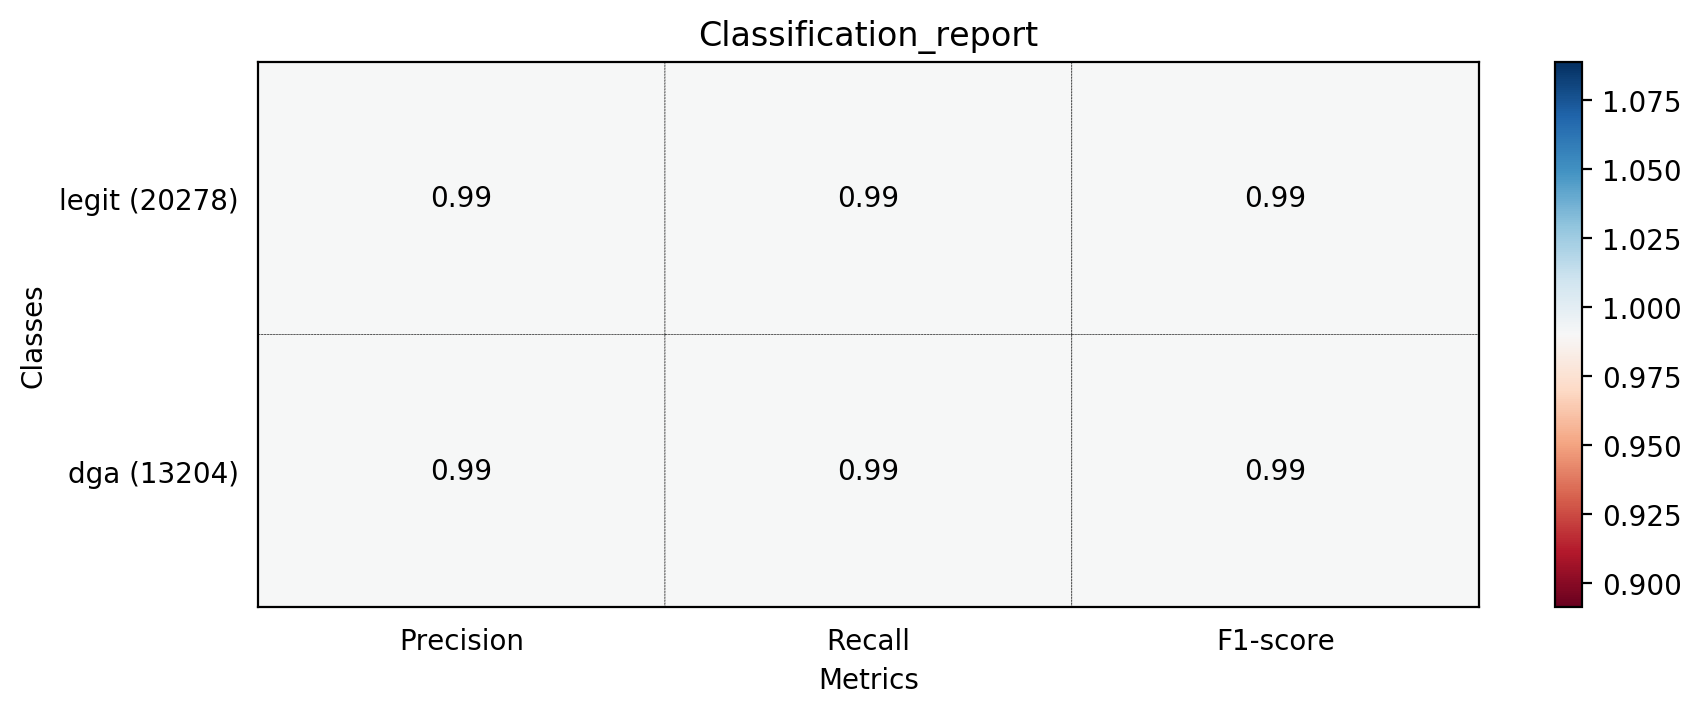
\includegraphics[width=.85\columnwidth]{figures/rndf_tra_nosup_nosup/class_rep.png}
    \caption{Classificatore Random Forest: Report di classificazione su un subset di domini reali (legit) e malevoli (DGA).\label{fig:repdga}}

    \centering
    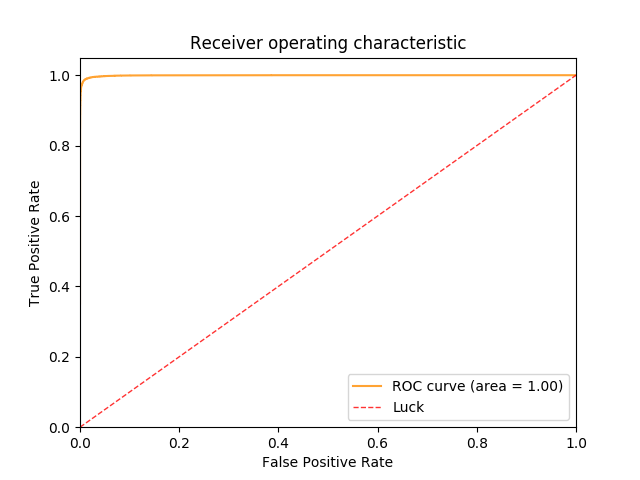
\includegraphics[width=.85\columnwidth]{figures/rndf_tra_nosup_nosup/roc_plot.png}
    \caption{Classificatore Random Forest: Area sottesa dalla curva ROC per il test con domini di tabella \ref{tab:malware}.\label{fig:rocdga}}
\end{figure}

In fase preliminare si è effettuato un confronto con altri due algoritmi di classificazione: SVC (C-Support Vector) e Gaussian Naive-Bayes. La loro performance non è stata altrettanto eccellente e pertanto si è deciso di accantonarli e proseguire con l'utilizzo di Random Forest. I report di classificazione sono mostrati in figura \ref{fig:repsvc} e \ref{fig:repgnb}.

\begin{figure}[htbp]
  	\centering
    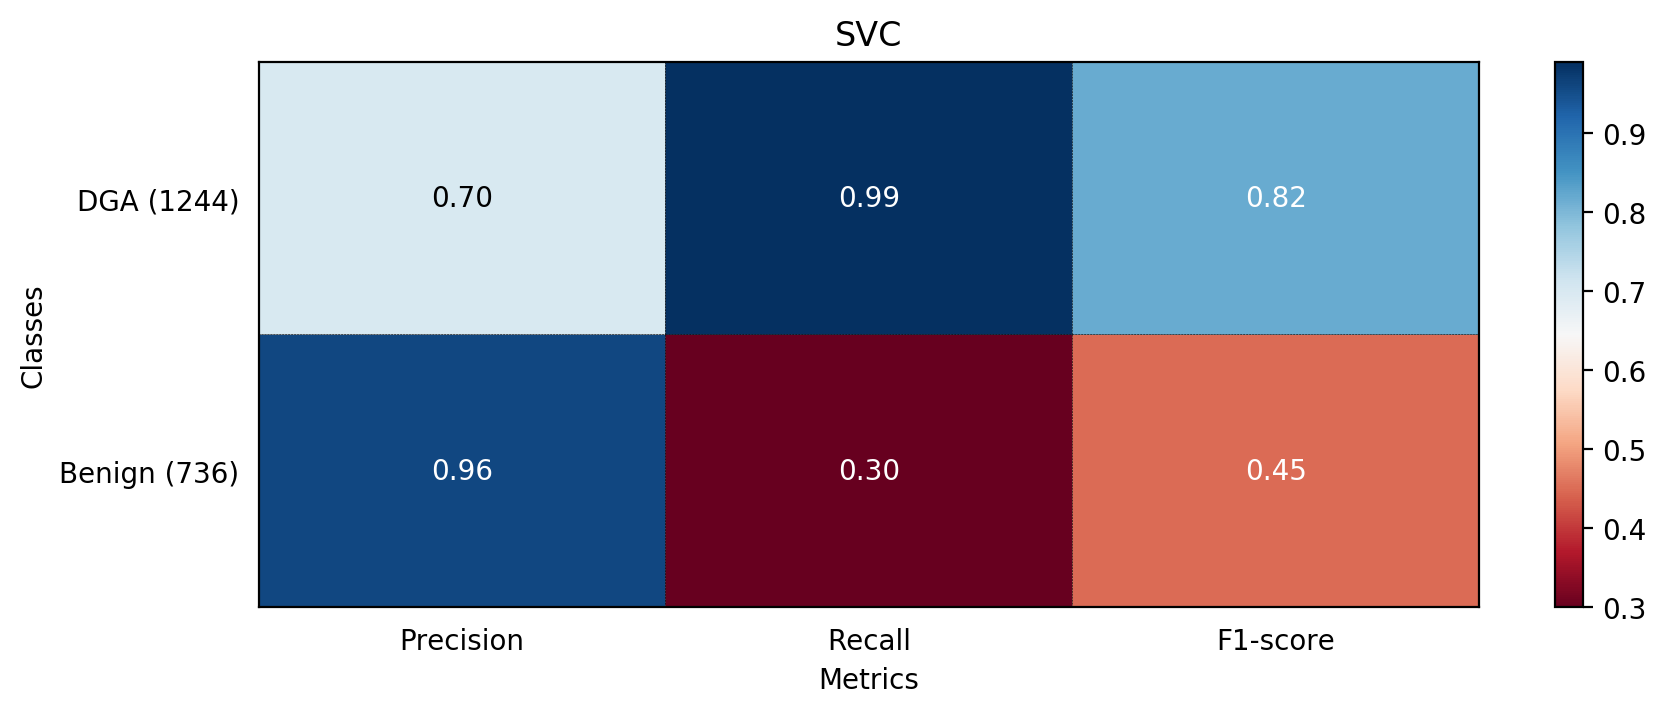
\includegraphics[width=.85\columnwidth]{figures/report_SVC.png}
    \caption{Report di classificazione per l'algoritmo SVC.\label{fig:repsvc}}

	\centering
    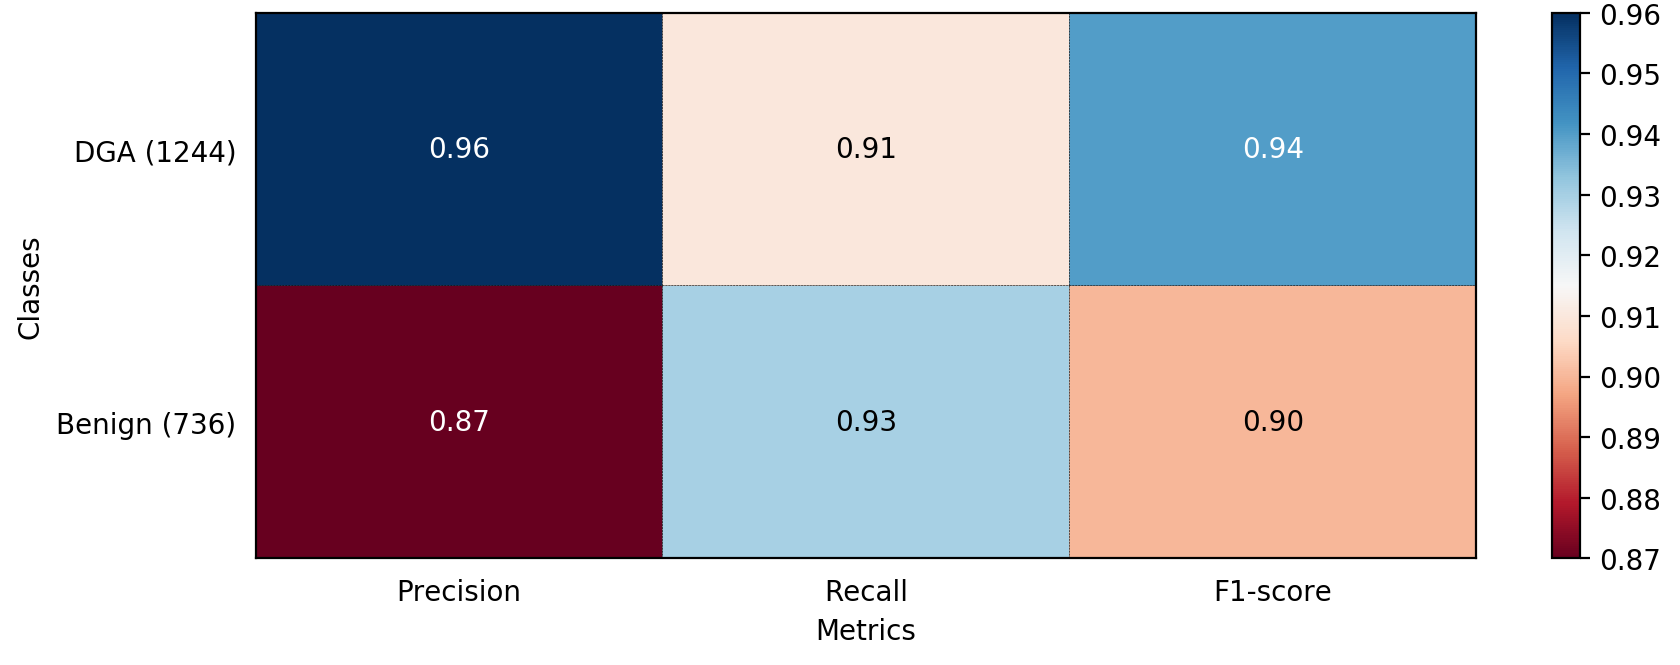
\includegraphics[width=.85\columnwidth]{figures/report_GaussianNB.png}
    \caption{Report di classificazione per l'algoritmo Gaussian Naive-Bayes.\label{fig:repgnb}}
\end{figure}

Il classificatore random forest è stato testato inserendo \textit{suppobox} tra le famiglie DGA già presenti. Si è scelto tale malware come campione esterno in quanto presenta la maggiore differenza rispetto alle famiglie mostrate in tabella \ref{tab:malware}. I risultati si possono vedere in figura \ref{fig:repsup} e \ref{fig:rocsup} e come si può notare la performance ne è fortemente influenzata, introducendo una grande percentuale di falsi nelle predizioni effettuate dal classificatore.

\begin{figure}[htbp]
    \centering
    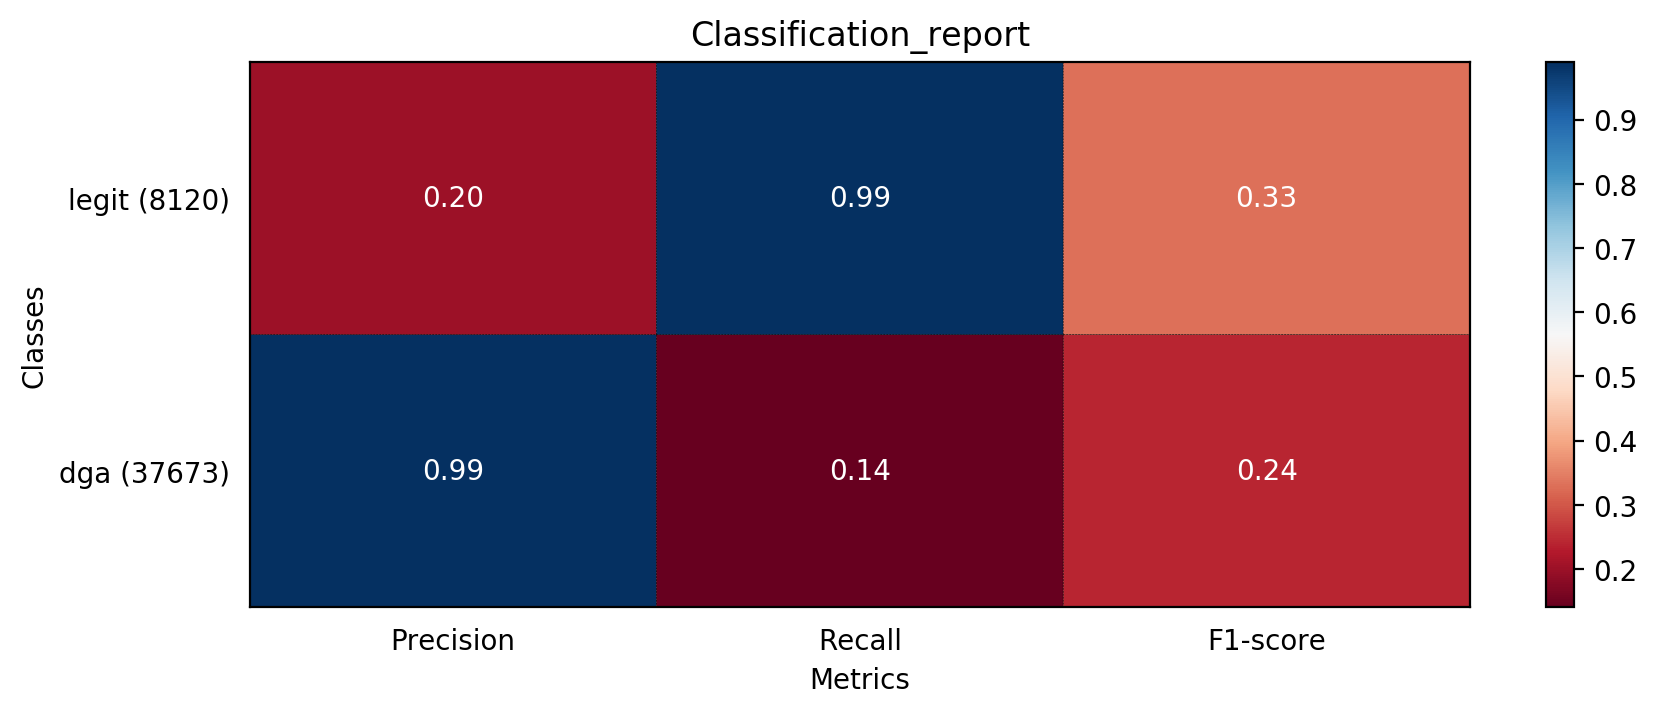
\includegraphics[width=.85\columnwidth]{figures/rndf_tra_nosup_sup/class_rep.png}
    \caption{Classificatore Random Forest: Report di classificazione su un subset di domini reali (legit) e malware, comprendenti suppobox (DGA).\label{fig:repsup}}

    \centering
    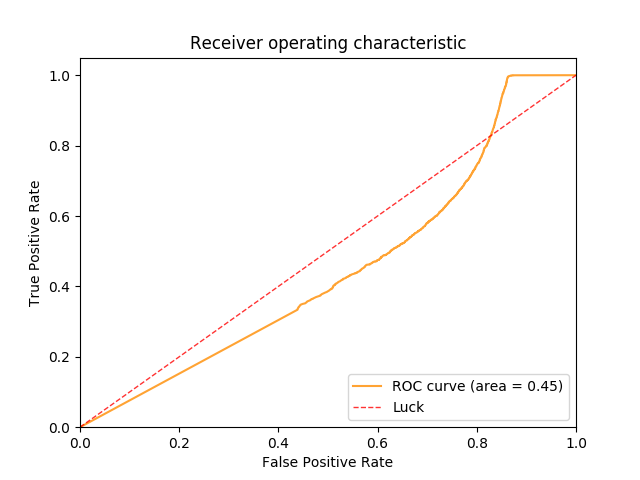
\includegraphics[width=.85\columnwidth]{figures/rndf_tra_nosup_sup/roc_plot.png}
    \caption{Classificatore Random Forest: Area sottesa dalla curva ROC per il test con  suppobox.\label{fig:rocsup}}
\end{figure}

\newpage
Come ultimo test è stato eseguito il training aggiungendo al precedente dataset di training una parte di domini generati da suppobox (Figura \ref{fig:repall} e \ref{fig:rocall}). Come si può notare la performance è migliorata sensibilmente, non raggiungendo comunque i risultati eccellenti del primo test.

\begin{figure}[!hb]
    \centering
    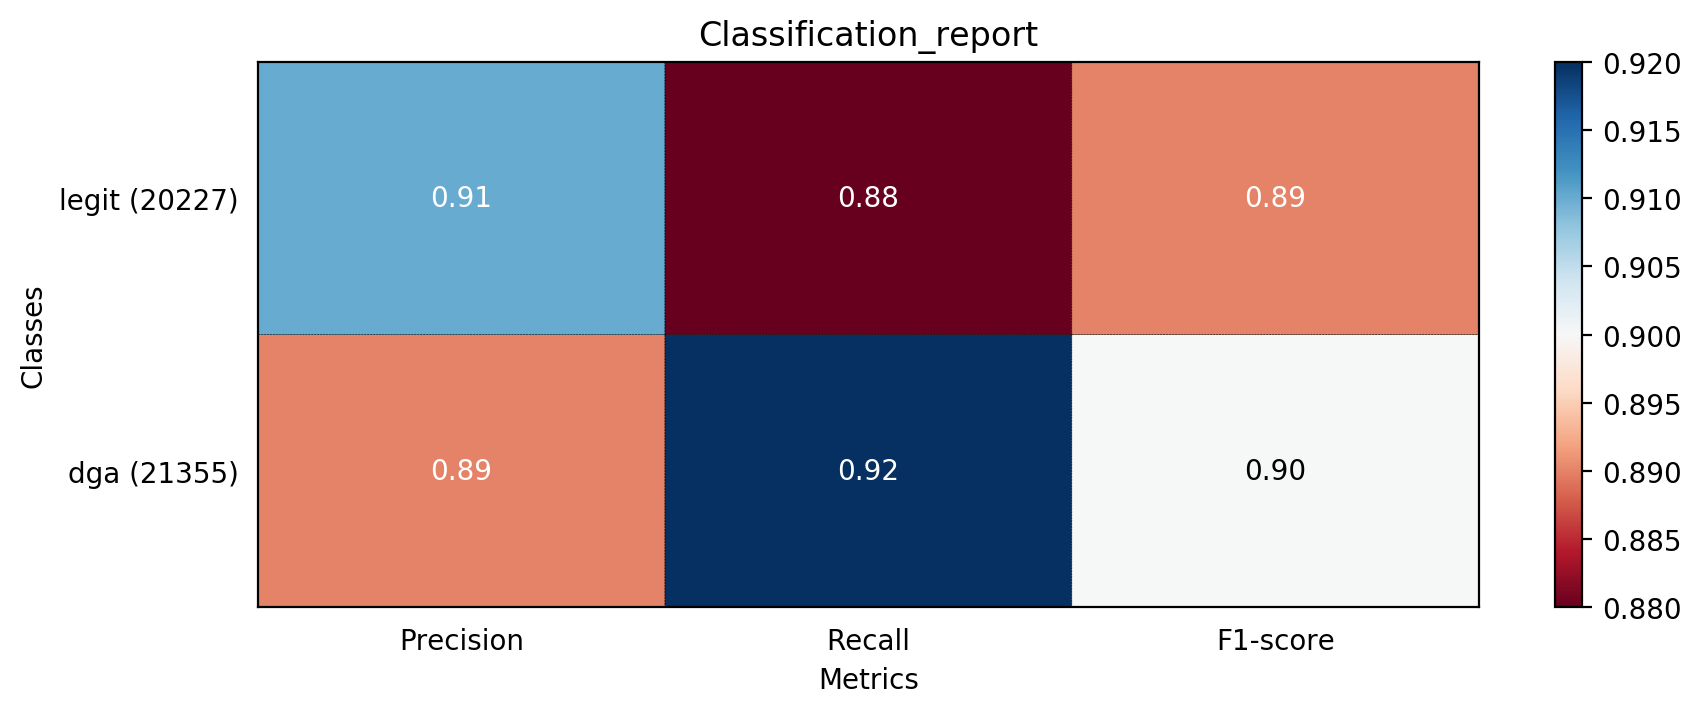
\includegraphics[width=.85\columnwidth]{figures/rndf_tra_sup_sup/class_rep.png}
    \caption{Classificatore Random Forest: Report di classificazione su un subset di domini reali (legit) e malware, comprendenti suppobox (DGA).\label{fig:repall}}

    \centering
    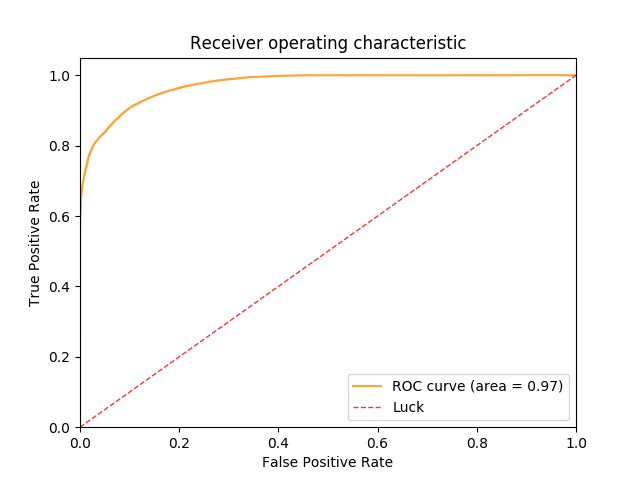
\includegraphics[width=.85\columnwidth]{figures/rndf_tra_sup_sup/roc_plot.png}
    \caption{Classificatore Random Forest: Area sottesa dalla curva ROC per il test con domini reali e malware (comprendenti suppobox).\label{fig:rocall}}
\end{figure}

\newpage
\section{Classificatore Neurale}
\label{ris:cnn}
Il classificatore neurale, nato per superare le mancanze del classificatore random forest, è stato testato nelle stesse condizioni utilizzate precedentemente: in particolare è stato utilizzato lo stesso dataset mostrato in sezione \ref{res:crf} e diviso ancora una volta in $\frac{9}{10}$ per la fase di training e $\frac{1}{10}$ per la fase di testing.

In prima fase si sono messe a confronto le tre architetture presentate in sezione \ref{classificatorenninterno}. Tali architetture hanno dimostrato tre andamenti simili; tuttavia a fronte dei risultati mostrati e della minore richiesta di risorse, il modello intermedio è risultato vincente rispetto agli altri testati. ( Figura \ref{fig:cfrmlp} )

\begin{figure}[!bp] 
\centering
	\begin{minipage}[t]{\linewidth}
		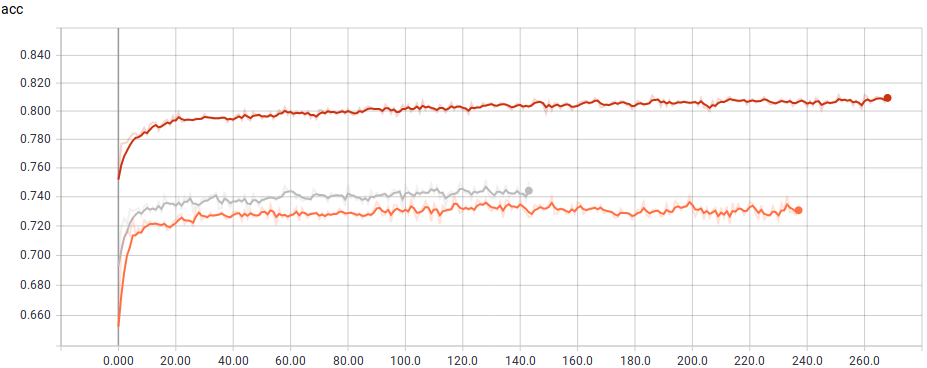
\includegraphics[width=\linewidth]{figures/MLP1.png}
	\end{minipage}\hfill
	\begin{minipage}[b]{\linewidth}
		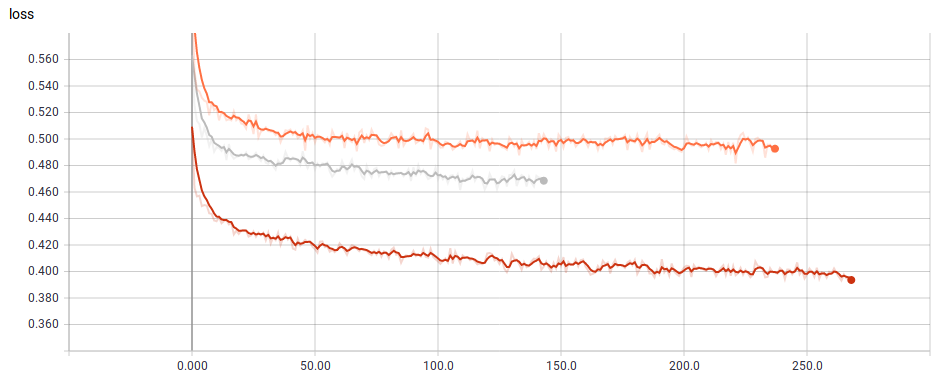
\includegraphics[width=\linewidth]{figures/MLP2.png}
	\end{minipage}
	\caption{Classificatore Neurale: Grafici di Accuracy e Loss  in funzione del tempo. confronto fra i tre modelli. La curva di colore grigio rappresenta il modello ingrandito, la curva di colore arancione rappresenta il modello ridotto mentre la curva di colore rosso rappresenta il modello intermedio; vincente tra i tre. \label{fig:cfrmlp}}
\end{figure}

Motivo di confronto è stata l'introduzione o meno di Batch Normalization \cite{1502.03167}. Come si può vedere dai grafici mostrati in figura \ref{fig:batchnorm} vi è una differenza di prestazione dovuta alla normalizzazione dei mini-batch, pertanto si è scelto di mantenere tale funzione all'interno dei livelli nonostante l'aumento di costi prestazionali.

\begin{figure}[!bp] 
	\begin{minipage}[t]{\linewidth}
		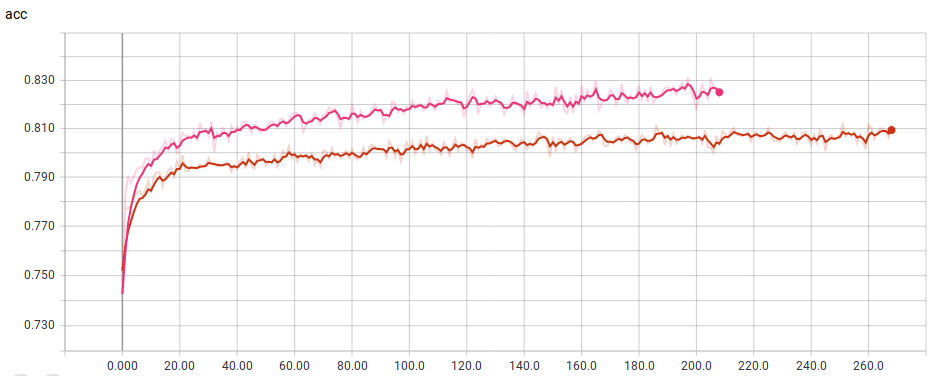
\includegraphics[width=\linewidth]{figures/MLP_batchnorm1.png}
	\end{minipage}\hfill
	\begin{minipage}[b]{\linewidth}
		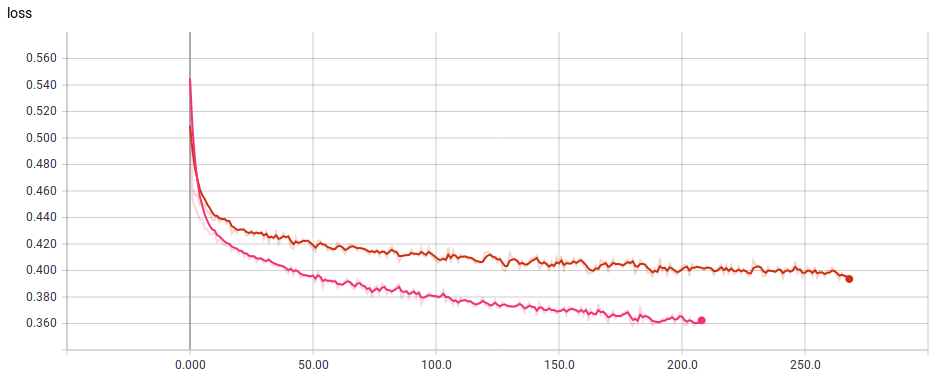
\includegraphics[width=\linewidth]{figures/MLP_batchnorm2.png}
	\end{minipage}
	\caption{Classificatore Neurale: Grafici di Accuracy e Loss in funzione del tempo per il modello intermedio. La curva rossa identifica il modello senza l'ausilio di Batch Normalization mentre la curva fuchsia rappresenta lo stesso modello con l'inserimento di Batch Normalization per ogni livello densamente connesso che compone il Multilayer Perceptron. \label{fig:batchnorm}}
\end{figure}

Particolarmente difficoltoso si è dimostrato il tuning degli  iperparametri di numero epoche e dimensione mini-batch per ottenere valori ottimali. Dopo una serie di test sperimentali che hanno messo a confronto diversi valori, si sono rilevati i valori
\begin{itemize}
\item \textbf{numero epoche} $= 60$
\item \textbf{dimensione minibatch} $= 35$ 
\end{itemize}

Tali valori hanno dimostrato di fornire la migliore performance durante la fase di training.

I test effettuati sul dataset hanno mostrato i risultati mostrati in figura \ref{fig:cnrepall} e \ref{fig:cnrocall}. Come si può vedere dai grafici il comportamento del classificatore è pressoché identico a quello mostrato dal classificatore random forest (figure \ref{fig:repall} e \ref{fig:rocall} )

\begin{figure}[!bp]
    \centering
    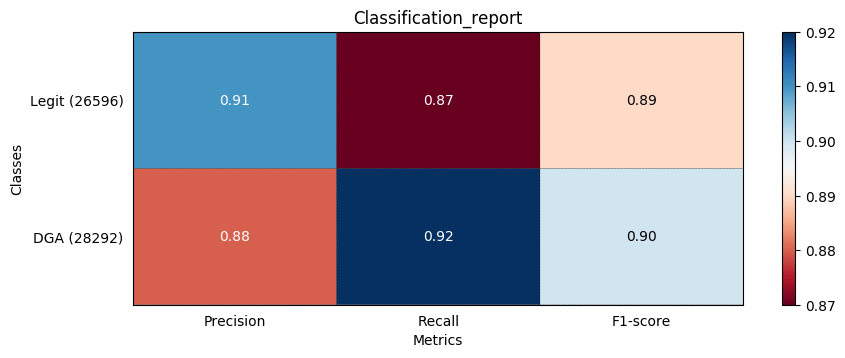
\includegraphics[width=.85\columnwidth]{figures/clas_nn/class_rep.png}
    \caption{Classificatore Neurale: Report di classificazione su un subset di domini reali (legit) e malware, comprendenti suppobox (DGA).\label{fig:cnrepall}}

    \centering
    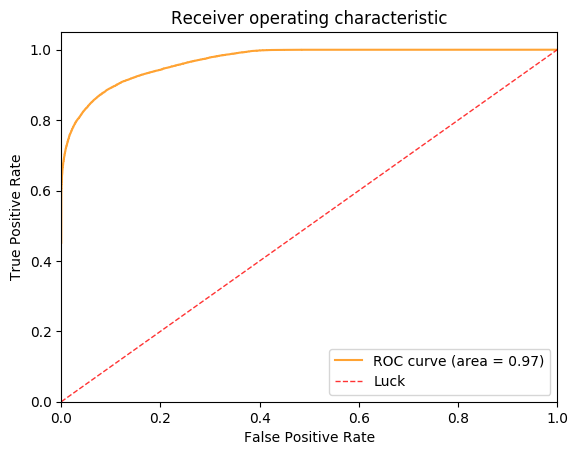
\includegraphics[width=.85\columnwidth]{figures/clas_nn/roc_plot.png}
    \caption{Classificatore Neurale: Area sottesa dalla curva ROC per il test con domini reali e malware (comprendenti suppobox).\label{fig:cnrocall}}
\end{figure}

A partire da questo classificatore neurale stabile è stato possibile implementare un sistema di adversarial learning tramite la GAN derivante da un autoencoder. 

\newpage
\section{Autoencoder}
\label{ris:autoenc}
L'autoencoder come presentato in sezione \ref{autoencoder} è stato testato con il dataset mostrato in sezione \ref{imp:autoencoder:dataset}. In fase sperimentale si è proceduto alla quantificazione della configurazione ottimale dell'autoencoder. In particolare si sono messi a confronto i valori di dropout presenti all'interno di encoder e decoder ed i valori di learning rate dei rispettivi compilatori. I valori finali di tali compilatori sono indicati all'interno della sezione \ref{imp:autoe:enc} e \ref{imp:autoe:dec}

In figura \ref{fig:aut1} e \ref{fig:aut2} è possibile notare i risultati della fase di training, per il quale si è trattenuto $\frac{1}{3}$ del training set come subset di validazione. Come è possibile notare l'ultima iterazione (colore verde) ha mostrato i risultati migliori e pertanto è stata utilizzata come base di partenza per il training della successiva GAN. 

L'utilizzo dei pesi dell'autoencoder come punto di partenza per il training della GAN ha contribuito fortemente a ridurre la instabilità di tale sistema, permettendo ai due sottosistemi generatore e discriminatore di partire da predizioni più precise rispetto all'utilizzo di pesi inizializzati in maniera randomica come generalmente attuato.

In tabella \ref{tab:autoenc} è possibile vedere un esempio di quali domini l'autoencoder produce dato un subset del dataset Alexa in input. Si può notare come siano vagamente simili ai domini reali per quanto riguarda la distribuzione dei caratteri e la lunghezza media dei domini, tuttavia non presenta ulteriori caratteristiche tali da influenzare negativamente i classificatori neurali.

\begin{table}[!hbp]
\centering
	\begin{tabular}{l}
	\toprule
	ehyt5tcncn3o5nw \\
	reknclkobg \\
	kne3xersl6npyr5 \\
	moeaamutlrhsn \\
	5t7-iitnvtrm5en \\
	r-zeotn0t-wuf \\
	bgargtas \\
	vviadammpielw \\
	7-aolelcfiextl \\
	morehekb \\
	\bottomrule
	\end{tabular}
	\begin{tabular}{l}
	\toprule
	d9ongedeo  \\
	meoomer \\
	zggy1lbxgi1psir \\
	ypsanilwrox \\
	bt5ennsl1zjchp0 \\
	runvpfcfrmaser \\
	anhgnxracokimoa \\
	atngsam \\
	de-poaz9yiiu \\
	nhntadt \\
	\bottomrule
	\end{tabular}
	\begin{tabular}{l}
	\toprule
	2kbth \\
	snd-drcepn \\
	sievd0 \\
	ono5ponlanafhic \\
	mmd0-5-ile \\
	su1aojp52 \\
	eraveok \\
	lfeubune \\
	ilnegban0 \\
	uim-rca0ohxmsbi \\
	\bottomrule
	\end{tabular}
	\begin{tabular}{l}
	\toprule
	oldohizlioczzu \\
	dodttiune \\
	ahoinin3 \\
	etiso9oo \\
	qi8gtuyte-ssg-n \\
	mlsrp8gf \\
	ktb1r2vb \\
	ptsdrqtanflog \\
	mcng5tsotnless \\
	rrhtsrceu \\
	\bottomrule
	\end{tabular}

\caption{Esempio di domini generati dall'autoencoder. \label{tab:autoenc}}
\end{table}

\begin{figure}[p]
    \centering
    \begin{minipage}[t]{0.7\linewidth}
    	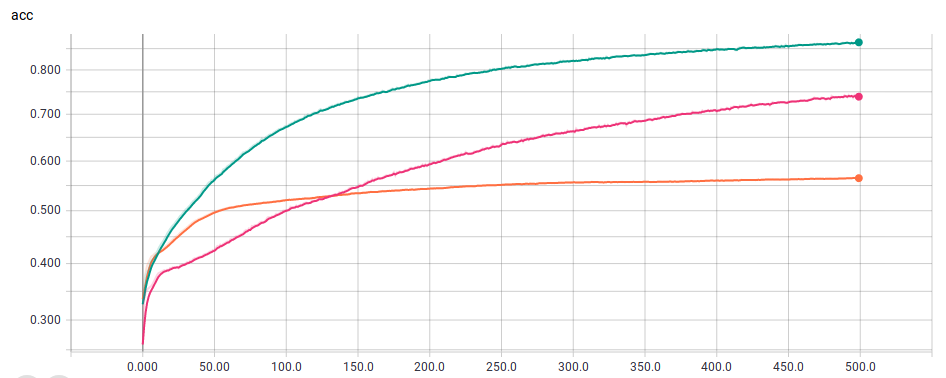
\includegraphics[width=\linewidth]{figures/autoenc.png}
    \end{minipage}\hfill
    \begin{minipage}[b]{0.7\linewidth}
    	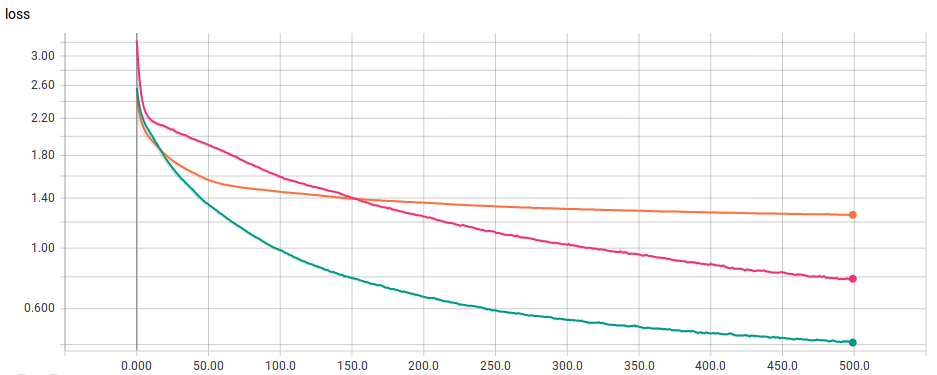
\includegraphics[width=\linewidth]{figures/autoenc2.png}
    \end{minipage}
    \caption{Grafici di Accuracy e Loss in funzione del tempo per la fase di training dell'autoencoder. La prima fase è rappresentata dalla curva arancione, la seconda dalla curva fuchsia mentre la terza fase è rappresentata dalla curva di colore verde. Si può notare come la terza iterazione raggiunga buoni valori di accuracy e loss; pertanto stato scelto come configurazione vincente per la GAN \label{fig:aut1}}
\end{figure}

\begin{figure}[p]
    \centering
    \begin{minipage}[t]{0.7\linewidth}
    	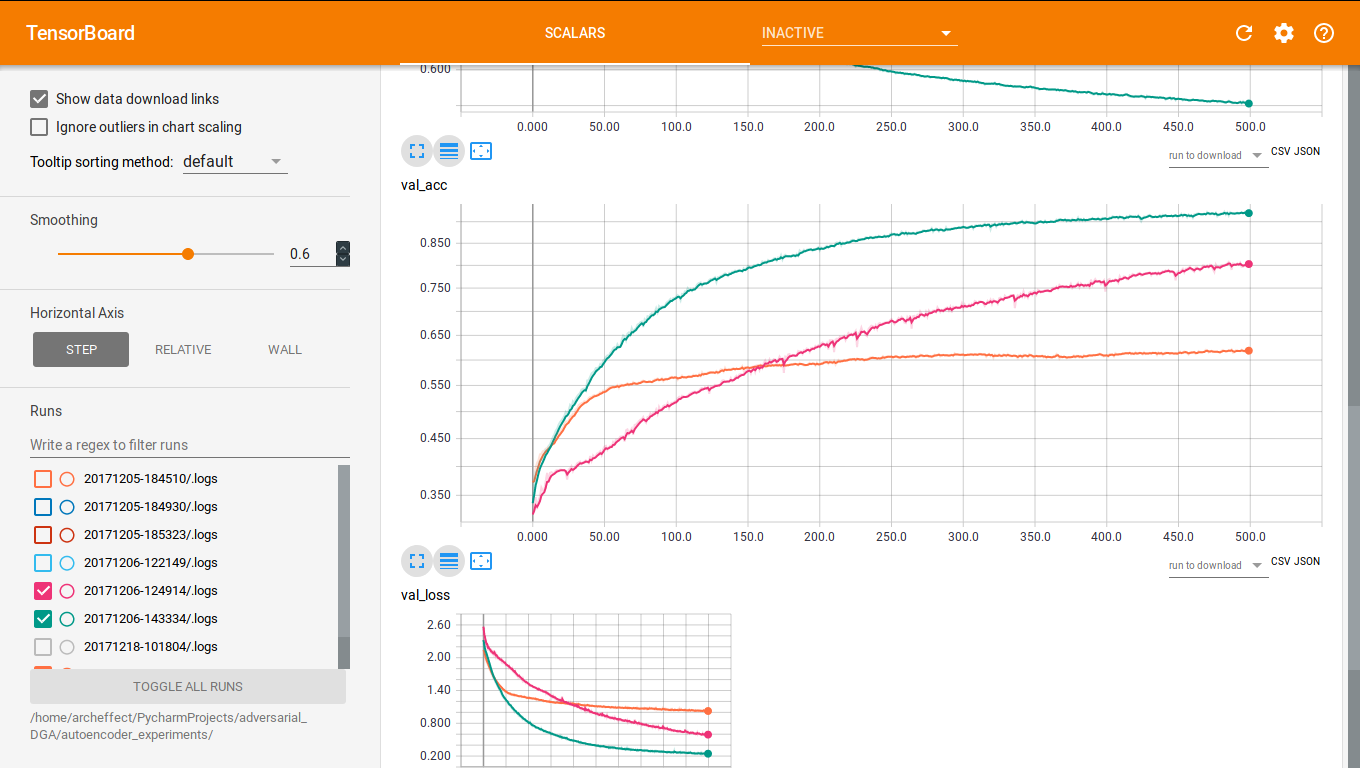
\includegraphics[width=\linewidth]{figures/autoenc3.png}
    \end{minipage}\hfill
    \begin{minipage}[b]{0.7\linewidth}
    	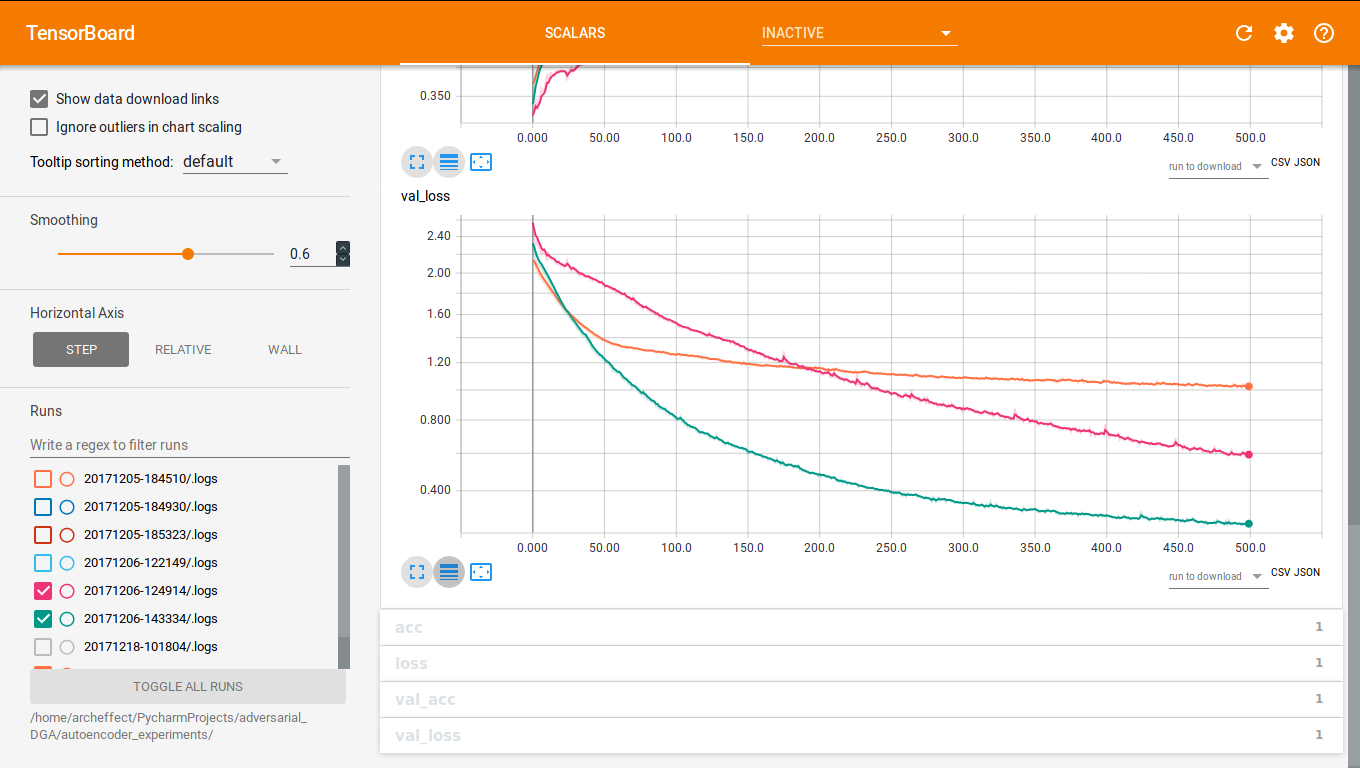
\includegraphics[width=\linewidth]{figures/autoenc4.png}
    \end{minipage}
    
\caption{Grafici di Accuracy e Loss in funzione del tempo rispetto al subset di validazione per la fase di training dell'autoencoder. Si può notare come i valori raggiunti siano molto simili a quelli ottenuti sul dataset di training, indice di qualità del modello rispetto a valori mai visti. \label{fig:aut2} }
\end{figure}

\newpage
\section{Generative Adversarial Network}
\label{ris:gan}
La Generative Adversarial Network descritta in sezione \ref{ganintro} e implementata come in sezione \ref{imp:gan} ha richiesto una lunga fase sperimentale nella quale è stato necessario trovare la giusta combinazione di iperparametri per i quali i due sottosistemi generatore e discriminatore potessero rimanere in equilibrio durante la durata necessaria per completare la fase di training. 

In particolare si sono incontrati due \textit{failure modes}:
\begin{itemize}
\item Caso in cui il discriminatore prevale sul generatore, come mostrato in figura \ref{fig:ganfailure1}, si ottiene una curva di \textit{loss} rasente lo zero, causando al generatore un incremento costante della propria curva di loss. Il significato di tale comportamento è l'impossibilità del generatore di generare domini sintetici sufficientemente realistici da poter mettere in crisi la predizione del discriminatore.
\item Caso in cui il generatore degeneri, producendo "spazzatura", rendendo eccessivamente semplice la predizione del discriminatore. La degenerazione infatti avviene in forma di domini generati tutti uguali, contenente una singola lettera ripetuta per tutta la lunghezza di caratteri. Tale comportamento è dovuto alla mancata capacità del generatore di mimare realisticamente i domini realistici. Un esempio di tale comportamento è mostrato in figura \ref{fig:ganfailure2}
\end{itemize}

\begin{figure}[!bp]
    \centering
    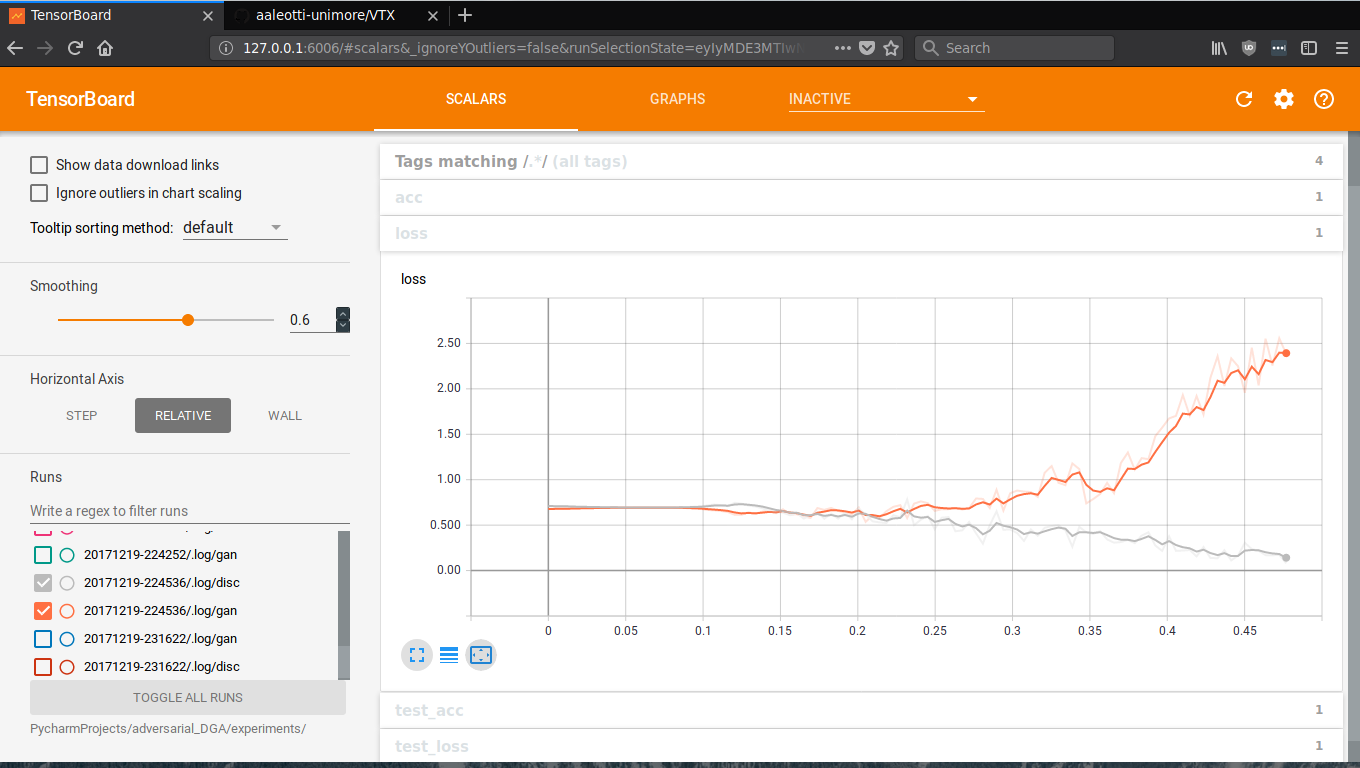
\includegraphics[width=0.6\columnwidth]{figures/gan/ganfailure1.png}
    \caption{Caso di degenerazione 1. Grafico del valore di loss in funzione del tempo. Il discriminatore (curva di colore grigio) prevale sul generatore (curva arancione), il quale non riesce a migliorare il proprio valore di loss.\label{fig:ganfailure1}}

    \centering
    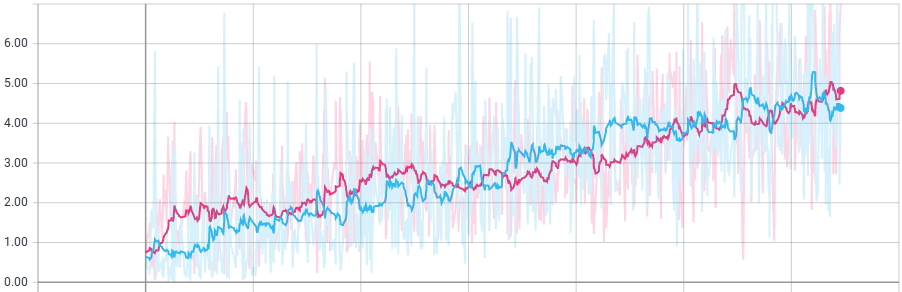
\includegraphics[width=.6\columnwidth]{figures/gan/ganfailure2.png}
    \caption{Caso di degenerazione 2. Grafico del valore di loss in funzione del tempo. Il generatore (curva di colore azzurro) non produce domini realistici, degenerando a dati inutilizzabili. Il discriminatore (curva di colore rosso) di conseguenza migliora la propria loss a causa della differenza sempre maggiore tra domini realistici e domini sintetici. \label{fig:ganfailure2}}
\end{figure}

E' stato possibile ottenere la stabilità della GAN, grazie a numerose tecniche empiriche ottenute da \cite{1606.03498} ed all'utilizzo del pre-training fornendo come inizializzazione i pesi ottenuti dalla fase di training dall'autoencoder. In figura \ref{fig:ganok} si può vedere l'andamento dei valori di loss di generatore e discriminatore nel caso di equilibrio tra le due reti neurali.

\begin{figure}[!bp]
\centering
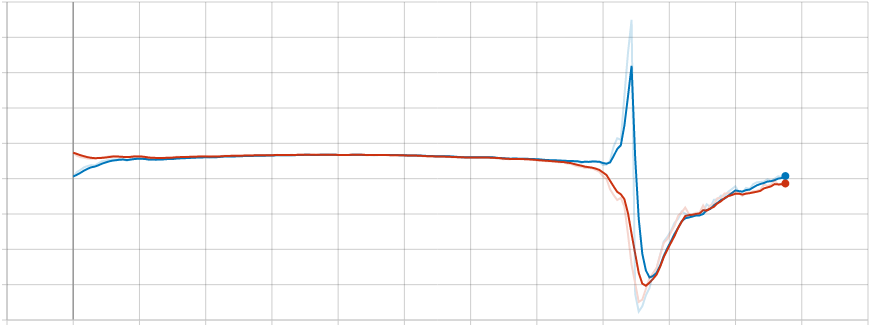
\includegraphics[width=\columnwidth]{figures/gan/ganok.png}
\caption{Grafico di loss in funzione del tempo per discriminatore (curva di colore rosso) e generatore (curva di colore azzurro). L'andamento rimane equilibrato fino al punto in cui il generatore non riesce a generare nuovi domini in grado di mettere in crisi il discriminatore. \label{fig:ganok}}
\end{figure}

Grazie a tale training è stato possibile infine generare un dataset di domini sintetici provenienti dalla GAN, che mimassero in maniera più precisa i domini realistici. Come si può notare in tabella \ref{tab:gan} 

\begin{table}[!bp]
\centering
	\begin{tabular}{l}
	\toprule
edarareve \\
skonasesosarere \\
skaran-unar \\
chicochophavock \\
dichoros \\
isherevores \\
nillersosersrsp \\
rldicde \\
escrarararuro \\
aemjtup \\
	\bottomrule
	\end{tabular}
	\begin{tabular}{l}
	\toprule
	ssrarsone \\
asccacca \\
monasheamc \\
itsusosose \\
stlega \\
ivortewrp \\
sdesedlsss \\
nggeneneres \\
madesadk \\
cesasasrrrrrrs \\
	\bottomrule
	\end{tabular}
	\begin{tabular}{l}
	\toprule
	horicicocr \\
sthonacorl \\
raocjcacarcrarl \\
vichitos \\
ogagagasuss \\
plerundinwoshn \\
odocococcocke \\
tuccronpcs \\
mivorthitdhud \\
mtuvocaro \\
	\bottomrule
	\end{tabular}
	\begin{tabular}{l}
	\toprule
avensdends \\
mwonwonerene \\
inihkkellgcrock \\
madoxto \\
ljarlers \\
maahofononoris \\
msusongere \\
scsacccca \\
rrngajiagjonggk \\
ituutasisa \\
	\bottomrule
	\end{tabular}

\caption{Esempio di domini generati dalla GAN. \label{tab:gan}}
\end{table}

\begin{figure}[!bp]
    \centering
    \begin{minipage}[t]{0.45\columnwidth}
		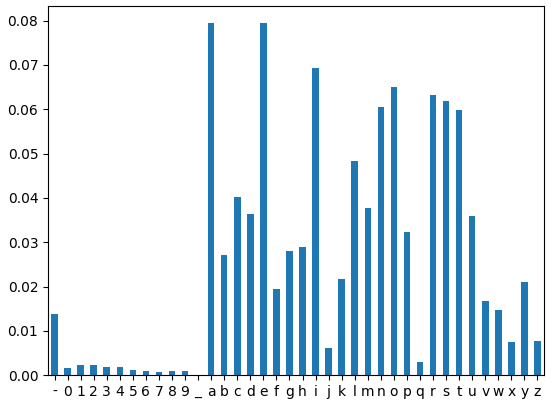
\includegraphics[width=\linewidth]{figures/all_legit_char_distr.png}
	\end{minipage}
	\begin{minipage}[b]{0.45\columnwidth}
		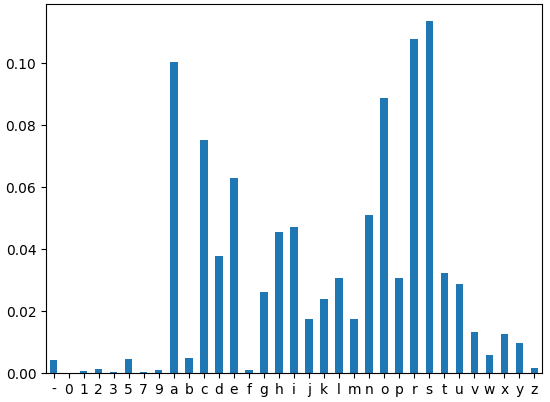
\includegraphics[width=\linewidth]{figures/chars_histogram.png}
	\end{minipage}
\caption{Confronto della distribuzione dei caratteri reali (grafico a sinistra) e generati algoritmicamente dalla GAN (grafico a destra) \label{fig:chardistr}}
\end{figure}


\begin{figure}[p]
    \centering
    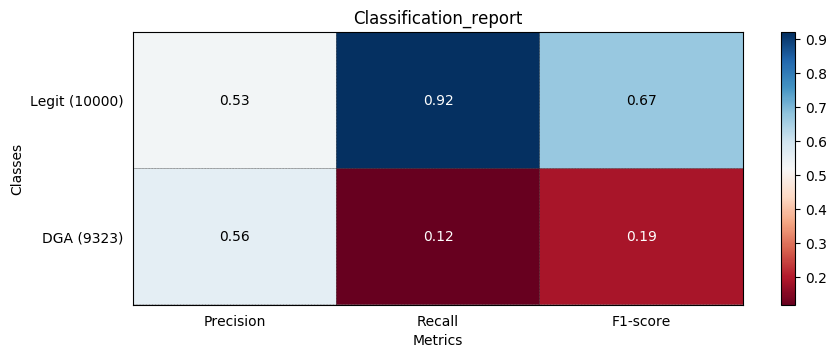
\includegraphics[width=\columnwidth]{figures/gan/class_rep.png}
    \caption{Classificatore Neurale testato su GAN: Report di classificazione su un subset di domini reali (legit) e generati da GAN (DGA).\label{fig:repgan}}

    \centering
    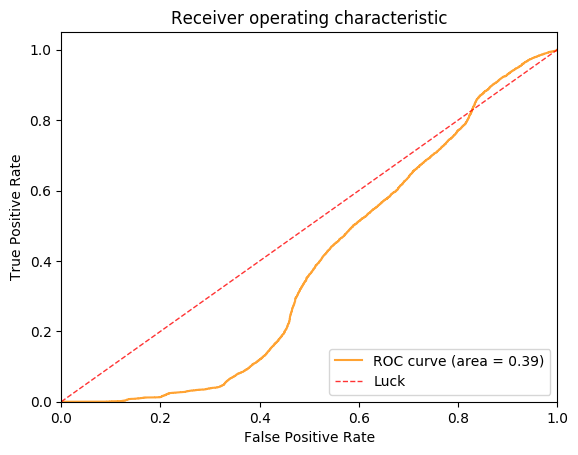
\includegraphics[width=\columnwidth]{figures/gan/roc_plot.png}
    \caption{Classificatore Random Forest: Area sottesa dalla curva ROC per il test con domini reali e generati da GAN.\label{fig:rocgan}}
\end{figure}
